\chapter{Premises}

\section{Preliminary reflections}\label{preliminary-reflections}

Music composition

What does it mean?

To compose, to assemble, to put together something.

Let's tackle some basic concepts about in no particular order.

\subsection{Concrete things}\label{concrete-things}

Before producing any sound we must choose or assemble a physical object.

\begin{center}
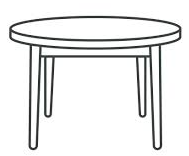
\includegraphics[scale=0.45]{../img/tavolo.png}
\end{center}

Pyhsical object with elestic characteristics can be exited in some way producing sound waves.

\begin{center}
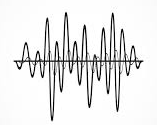
\includegraphics[scale=0.55]{../img/pelle.png}
\end{center}

Sound waves are a form of energy that propagates in time and space through an elastic medium.

Sound waves simply exist in our world.

When a sound wave reaches our ears it is perceived as an acoustic information by our brain.

\begin{center}
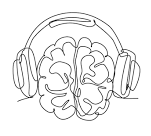
\includegraphics[scale=0.5]{../img/percezione.png}
\end{center}

It's a concrete thing.

When it was choosen or assembled:

\begin{itemize}
\tightlist
\item we can interact with it (touch it, move it, etc.).
\item we can make a copy (a model).
\item we can modify it (improve it).
\item we can destroy (or forgot) it.
\item it does not require linguistic representation, it simply be.
\item it exist in space and not necessary in time.
\end{itemize}

This has to do with the physical world.

We live immersed in sound waves.

We listen to music more or less daily but\ldots is music always sound waves?

No.

We can think and organize sounds inside our mind without producing them as sound waves.

\begin{center}
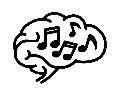
\includegraphics[scale=0.65]{../img/musicervice.png}
\end{center}

Sound waves have to do with physical world and human perception.

Music is a complex thing that has to do with both perceptual and cognitive human systems.

\subsection{Pre-linguistic}\label{pre-linguistic}

We can compose ideas or instinctive sequences of sounds.

Putting thoughts together in a pre-linguistic manner.

\begin{center}
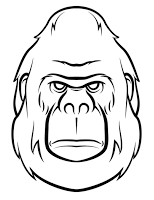
\includegraphics[scale=0.35]{../img/pensiero.png}
\end{center}

An abstract thing.

When we thinked it:

\begin{itemize}
\tightlist
\item we can't interact with it (touch it, move it, etc.).
\item we can do a copy (replicate pattern structure).
\item we can reproduce it but only in its physical forms (kinds of matter):
   \begin{itemize}
   \tightlist
   \item declaiming it (sound waves).
   \item writing it on a paper using symbolic representations.
   \end{itemize}
\item we can modify it.
\item we can't destroy it (we can only destroy its representation in physical world - book, recordings, etc. - not in our memory).
\item it does not require linguistic representation.
\item it exists in the space of consciousness (our mind) but when we
  reproduce it in the physical world it exist both in space and time.
\end{itemize}

This has to do with mind, consciousness and human expression.

Let's explore this concept through a comparison between natural language and musical language because they: 
\begin{itemize}
\tightlist
\item are universal (present in all human cultures). 
\item belong exclusively to our species. 
\item ensure the cohesion of a social group. 
\item share formal and functional characteristics.
\end{itemize}

\subsubsection{Natural language}\label{natural-language}

Psycholinguistic studies say that at a deep level all natural languages have the same structure and this can tell us something universal about the human intellect (our brain).

The form of human thought is innate and common to all members of the species.

The function of language is to express it.

\begin{center}
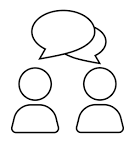
\includegraphics[scale=0.5]{../img/linguaggio.png}
\end{center}

The deep structure of an expression is closely related to the thought it represents.

If pre-linguistic thoughts have the same type of form for everyone the linguistic structures that represent them must also have the same type of form.

\begin{center}
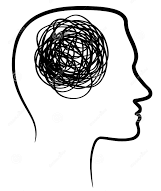
\includegraphics[scale=0.4]{../img/prelinguistico.png}
\end{center}

If we want to transform a deep thought structure into a statement we assemble it together into a linear sequence of sounds.

This sequence must convey to the listener the necessary informations for its comprehension.

Thought itself cannot be considered a linguistic sequence because it exists independently of language.

\subsubsection{Musical language}\label{musical-language}

About music there exist forms of mental activity independent of any musical language such as \href{http://www.musicaecodice.it/gitmedia/emc/1_media/bimbi.mp3}{children's nursery rhymes} or \href{http://www.musicaecodice.it/gitmedia/emc/1_media/tibet.mp3}{tibetan songs}.

Pre-linguistic musical thought must be an abstract scheme that includes exclusively the characteristics common to all musics.

If both music language and natural language are universal characteristics of the human specie this means that humans have a natural capacity to acquire both linguistic and musical skills.

Natural language and musical language expressions are conveyed in the real world in the form of sound waves.

The sound waves common basic physical parameters are: 

\begin{itemize}
\tightlist
\item frequency \(\rightarrow\) interval, pitch, intonation. 
\item amplitude \(\rightarrow\) dynamic. 
\item time \(\rightarrow\) rhythm. 
\item timbre \(\rightarrow\) instrumental techniques, vocal expressions, orchestration.
\end{itemize}

Even though surface forms differ from culture to culture we can find these universal elements not only in physical parameters but also in the subdivision into multiple levels of the languages.

\subsection{Compose a phone number}\label{compose-a-phone-number}

\begin{center}

\includegraphics[scale=0.4]{../img/telefono.png}
\end{center}

Defining a code.

\begin{itemize}
\tightlist
\item a sequence of numbers (or letters or sounds) that represents a thought.
\item we can't modify it.
\item it requires encoding and decoding.
\item to understand it we need to know its linguistic structure.
\item it follow precise and shared rules.
\item if we don't know them, the sequence of numbers or sounds makes no sense to us.
\item it require linguistic representation.
\item it can be: 
  \begin{itemize}
  \tightlist
  \item in space \(\rightarrow\) if you write it in a phone directory.
  \item in time \(\rightarrow\) if you digit it on a phone keyboard.
  \end{itemize}
\end{itemize}

This has to do with language and its representations.

Let's start again with the comparison between natural and musical language.

Leaving aside the first common level represented by the physical parameters of sound both are built on further different levels.

Simplifying, we can identify four levels:

\begin{itemize}
\tightlist
\item phonetic-phonological \(\rightarrow\) phonetics and prosody - individual notes, pitches, scales, tunings, etc.
\item morphosyntactic \(\rightarrow\) combination of phonemes into morphemes and morphemes into words - rhythm, chords, etc.
\item syntactic \(\rightarrow\) rules defining the relationships between words - counterpoint, harmony, twelve-tone system, asides, phrases, etc.
\item semantic \(\rightarrow\) access to meaning.
\end{itemize}

\subsubsection{Phonetic-phonological level }\label{phonetic-phonological-level}

It is present in all languages.

Every linguistic output can be broken down into phonemes which are a small set of sound classes.

For example the word `ape' is made up of three phonemes one for each letter.

Phonemes have two distinctive features: 

\begin{itemize}
\tightlist
\item they are not characterized by absolute values but by a set of sounds within a certain range. 
\item the continuum of sounds is divided differently in different languages (two sounds that constitute two phonemes in one language form a single phoneme in another).
\end{itemize}

\begin{center}
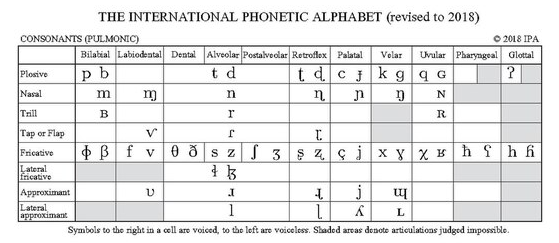
\includegraphics[scale=0.9]{../img/fonemi_2.png}
\end{center}

In western musical languages the fundamental phoneme could be considered the note with its various types of expression (staccato, tenuto, accentato, legato, etc.).

\begin{center}
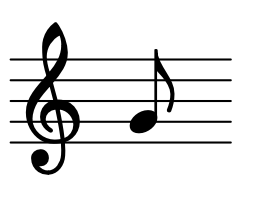
\includegraphics[scale=0.22]{../img/nota.png}
\end{center}

Let us remember that in both languages they are characterised by frequency, duration, amplitude and timbre.

\subsubsection{Morphosyntactic level }\label{morphosyntactic-level}

Phonemes can join together to form morphemes.

Morphemes can join together to form words.

Words are basic elements of language that: 

\begin{itemize}
\tightlist
\item carries meaning. 
\item can be used on its own.
\item are uninterruptible.
\end{itemize}

In music we could consider them as a short melodic pattern (inciso).

\begin{center}
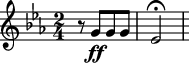
\includegraphics[scale=0.7]{../img/inci.png}
\end{center}

A vocabulary (lexicon) is a set of words in a given language.

In music we could consider it as a set of rhytmic and melodic patterns.

Substantial differences between the two languages:

\begin{itemize}
\tightlist
\item in natural language a word has a general function (the word `table' represent a table).
\item in music a specific word exist only within a piece (we can consider Beethoven's fifth symphony incise a word only in this symphony).
\end{itemize}

\subsubsection{Syntactic level }\label{syntactic-level}

Syntax or formal grammar \(\rightarrow\) a closed system of rules that serves exclusively to generate the set of sequences considered grammatical.

Every natural language like every musical language has its own syntax (Italian, French, German, counterpoint, harmony, twelve-tone, etc.).

We have previously defined that music is not necessarily conveyed through sound waves but\ldots are sound waves always music?

No, again.

In order to be defined music language requires a codification of sounds in vocabularies and systems of rules.

\begin{center}
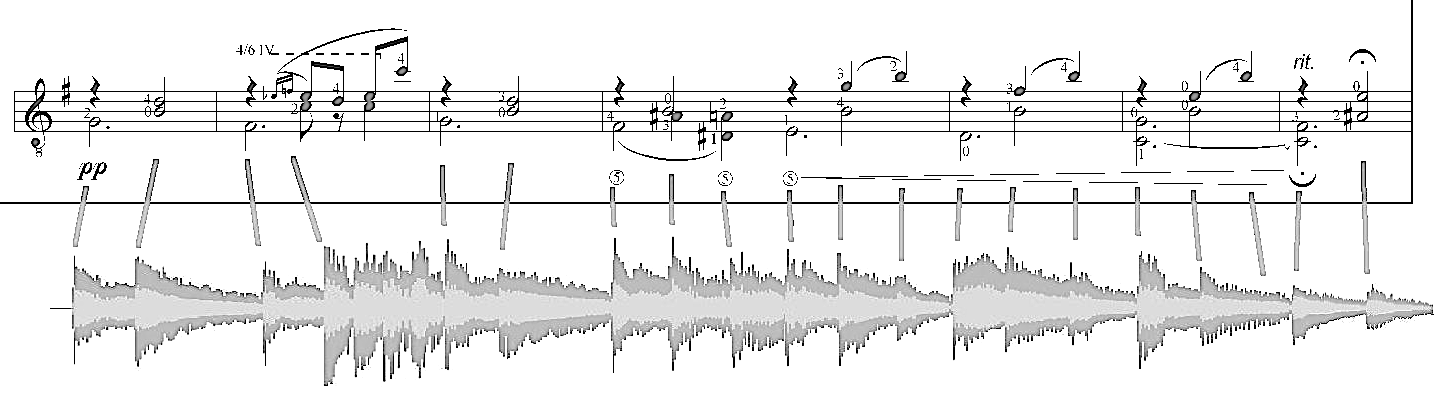
\includegraphics[scale=0.9]{../img/ondenote.png}
\end{center}

In all musical cultures the physical parameters of sound are organized in symbols.

These symbols can become independent from sound waves.

\begin{center}
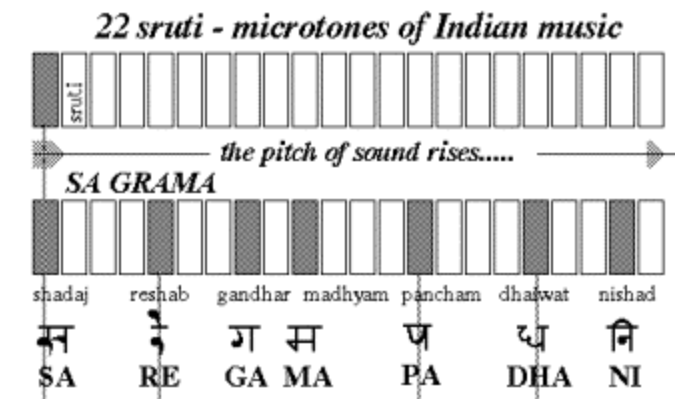
\includegraphics[scale=0.4]{../img/india.png}\break
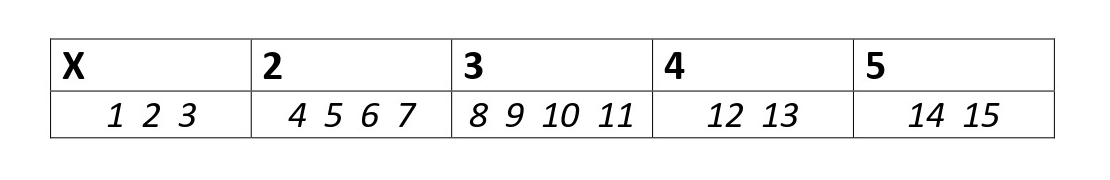
\includegraphics[scale=0.3]{../img/rtmoindia.png}
\end{center}

In Western musical tradition, from psamody until around 1940 these parameters have maintained more or less the same vocabulary over the centuries (diatonic and chromatic intervals, metric and subdivision of beat, musical instruments, etc.).

\begin{center}
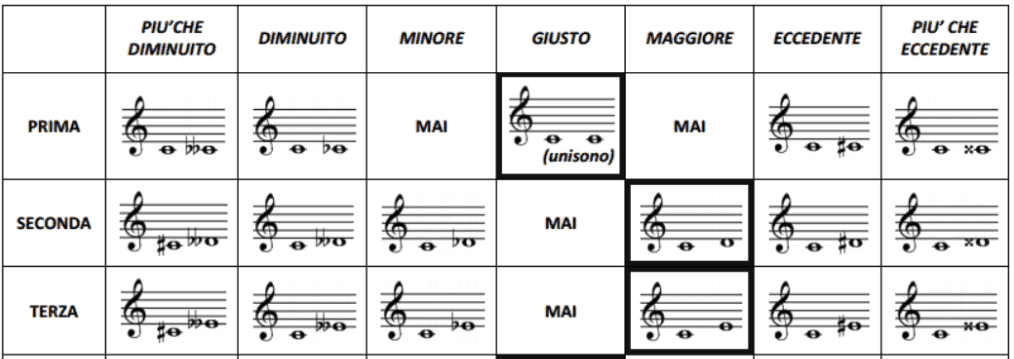
\includegraphics[scale=0.85]{../img/intervalli.png}
\end{center}

The systems of rules through which the vocabulary terms were organized (syntax), however, were different (modality, counterpoint, harmonic systems, dodecaphony, stocastic systems, alea, etc.).

\begin{center}
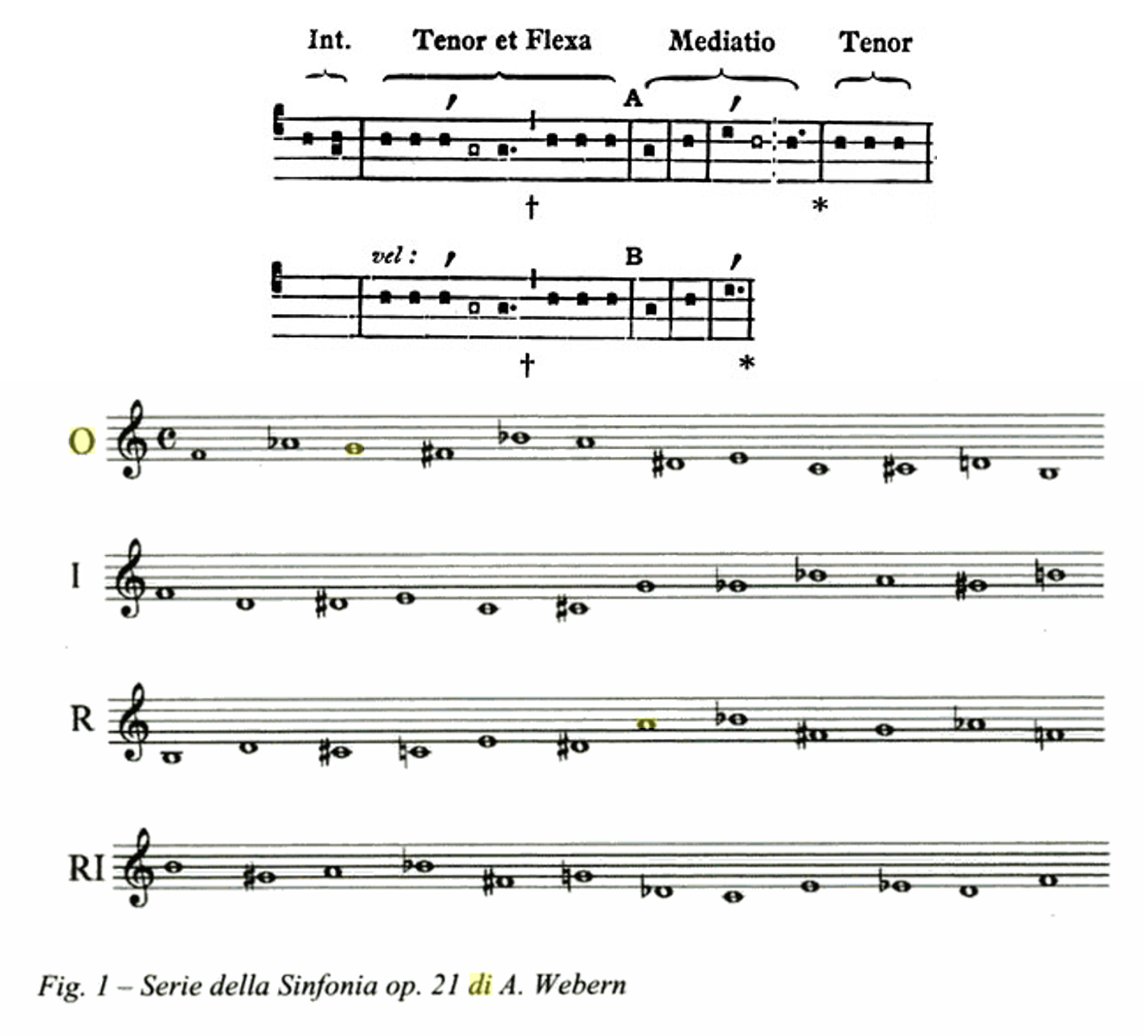
\includegraphics[scale=0.75]{../img/greg.png}
\end{center}

For this reason we cannot define western music as a single language but as a set of languages \hspace{0pt}\hspace{0pt}that use the same vocabulary (classical music, baroque music, pop music, jazz music, etc.).

Even more so if we talk about music from different cultures.

On this level the differences underlined at the end of the previous paragraph regarding musical words disappear.

Musical grammars are a meta-reflection that deals with symbolic forms.

These can be abstracted to the point of taking on a meaning of their own that goes beyond the perception of the work.

\begin{center}
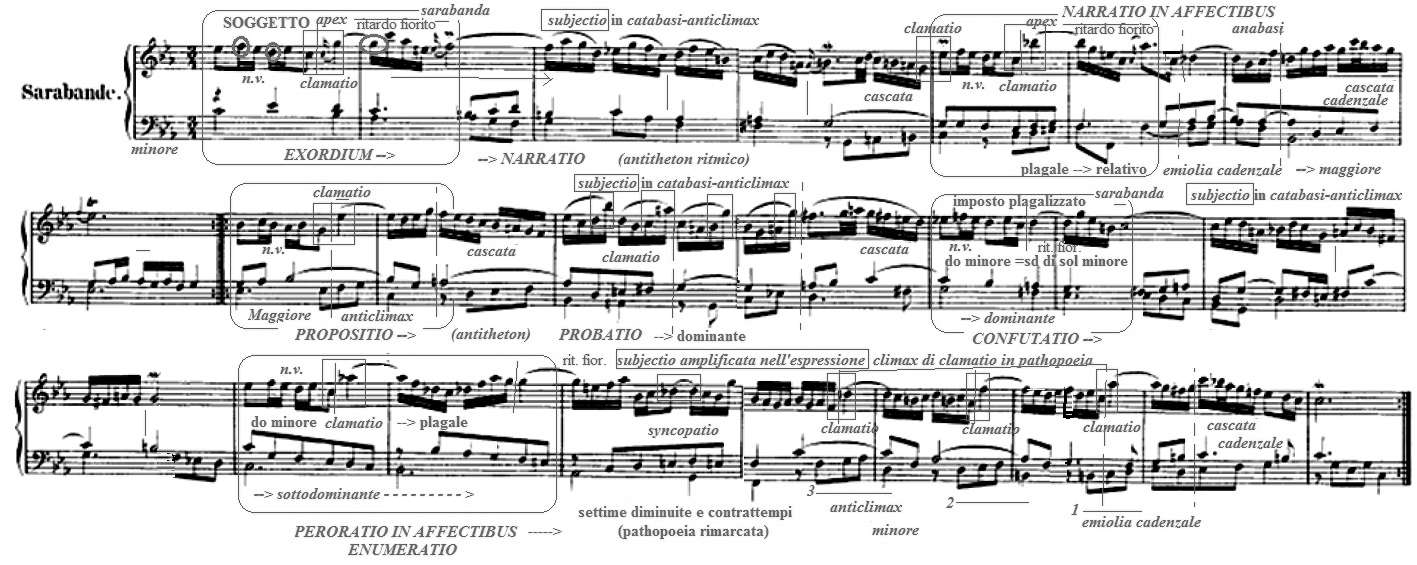
\includegraphics[scale=1.1]{../img/analisische.png}
\end{center}

\subsubsection{Semantic level}\label{semantic-level}

The branch of linguistics and logic concerned with meaning.

In musical language there are several starkly contrasting theories on this subject none of which can be assumed to be universal.

The one that summarizes the two main positions was proposed by the American musicologist L.B.Meyer who distinguishes between two forms of meaning in music:

\begin{itemize}
\tightlist
\item designative meaning \(\rightarrow\) which refers to something extramusical (G.Malher \href{http://www.musicaecodice.it/gitmedia/emc/1_media/malher.mp3}{Symphony n 10} - extract).
\item embodied meaning \(\rightarrow\) the meaning a piece has for the listener in terms of:

  \begin{itemize}
  \tightlist
  \item Internal syntactic structure.
  \item Interactions between this structure and the listener's musical knowledge and expectations. Musical structure can create expectations that can be disappointed or fulfilled generating a dynamic flow of tensions and resolutions that influence the listener's emotional and aesthetic responses. These are aesthetic emotions that have nothing to do with the emotions experienced in real life (F.Schubert \href{http://www.musicaecodice.it/gitmedia/emc/1_media/schubert.mp3}{Trio} - extract).
  \end{itemize}
\end{itemize}

Can we express in words what emotions listening to this Schubert trio arouses in us?

We will delve deeper into this last topic in the \hyperref[meaning]{Music’s meaning} section.

These levels enable common phenomena that help us understand the difference between sound waves and language.

\begin{itemize}
\tightlist
\item categorical perception \(\rightarrow\) a continuous linguistic or musical sound is segmented into discrete categorized units (phonemes, notes, words). If we repeat the same phrase or melody several times they will always be recognized as the same despite variations in acoustic parameters sometimes even significant ones (\href{http://www.musicaecodice.it/gitmedia/emc/1_media/pollini.mp3}{exemple 1}, \href{http://www.musicaecodice.it/gitmedia/emc/1_media/kissin.mp3}{exemple 2}, \href{http://www.musicaecodice.it/gitmedia/emc/1_media/sokolov.mp3}{exemple 3}).
\item phonemic restoration \(\rightarrow\) replacing part of the linguistic signal with noise simultaneously with the word or music does not affect the perception of the whole. Semantic-lexical or musical expectations prevail over acoustic analysis (\href{http://www.musicaecodice.it/gitmedia/emc/1_media/buchi.mp3}{musical},  \href{http://www.musicaecodice.it/gitmedia/emc/1_media/vian.mp3}{natural}).
\item expectations \(\rightarrow\) the syntactic construction of a sentence leads us to expect one word rather than another within it, just as happens within a sequence of chords in tonal terms (\href{http://www.musicaecodice.it/gitmedia/emc/1_media/analisi.mp3}{words}, \href{http://www.musicaecodice.it/gitmedia/emc/1_media/accordi.mp3}{chords}).
\end{itemize}

\subsection{Perceive and process }\label{perceive-and-process}

The ability to perceive and process musical information (not exclusively acoustic) is also common to all cultures.

Listening to music from one's own culture provides the listener with additional implicit information.

The simplest musical competence requires the activation of numerous cognitive abilities, including: 

\begin{itemize}
\tightlist
\item memory \(\rightarrow\) short-term recognition of melodic rhythmic patterns.
\item maintenance of attention \(\rightarrow\) active listening.
\item analysis of the temporal structure \(\rightarrow\) continuous comparison between present and short-term memory.
\end{itemize}

These abilities are part of a body of knowledge acquired through more or less conscious implicit learning that occurs through two modalities:

\begin{itemize}
\tightlist
\item universal cognitive mechanisms \(\rightarrow\) experimental psychology studies have shown that even prenatally the fetus responds to sounds and noises that activate phonological priming processes. For example, infants have been found to prefer sounds or stories frequently reproduced by their mothers after the third month of pregnancy over
those they have never heard. Even in adulthood, some research has highlighted the existence of perceptual mechanisms independent of cultural context.

\item environmental and cultural interaction \(\rightarrow\) constant, quantitatively preponderant, continuous and more or less conscious perception of sounds organized according to the reference syntax of the cultural environment of reference.
  
\begin{center}
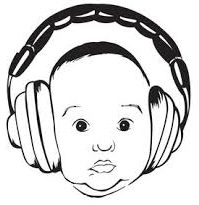
\includegraphics[scale=0.28]{../img/prenatale.png}
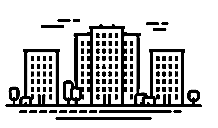
\includegraphics[scale=0.55]{../img/metro.png}
\end{center}
\end{itemize}

An example of the dichotomy just described can be found in analyzing the pitches of a melody.

To accomplish this we must activate several cognitive mechanisms which, in their simplest form are:

\begin{itemize}
\tightlist
\item processing the melodic profile (the progression of the ups and downs)  \(\rightarrow\) occurs more easily in both children and adults, with or without musical experience or literacy.
\item processing musical intervals (the distance between pitches) \(\rightarrow\) occurs less easily in general and to a greater extent in individuals with more experience or musical literacy (\href{http://www.musicaecodice.it/gitmedia/emc/1_media/veloso.mp3}{melody}).
\end{itemize}

\subsection{Re-compose a puzzle}\label{re-compose-a-puzzle}

\begin{center}
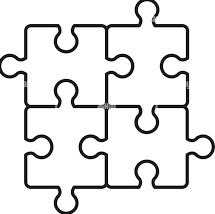
\includegraphics[scale=0.3]{../img/puzzle.png}
\end{center}

Re-constructing an image.

An abstract thing reconstructed in the physical world through a sequence of actions.

\begin{itemize}
\tightlist
\item we continuously interact between abstract and real world through attempts to correctly reproduce the original image.
\item we can reproduce the process many times but we cannot consider them copies.
\item we can't modify it.
\item it does not require necessary linguistic representation but cognitive skills.
\item during the re-composition process it need time and space but when the process is ended it need only space (in the case of a musical reproduction a space in our memory and consciousness).
\end{itemize}

This has to do with music representations, interpreters, players and performers.

Up to now we have thought about sound, music and their perception but not about the actors involved in the process of making music.

\begin{itemize}
\tightlist
\item composer.
\item interpreter.
\item listener.
\end{itemize}

We will delve deeper into these concepts in a dedicated paragraph \textit{Forms of human expression}.

\section{Music's meanings }\label{musics-meanings}

When we talked about the semantic level we mentioned the meaning but\ldots what is the meaning of music and what does music represent for humans?

We start again with sound waves \(\rightarrow\) it represent music in the physical world like clouds or mountains.

This has to do with both perceptual and cognitive processes.

By abstraction we can consider sound waves as \href{http://www.musicaecodice.it/gitmedia/emc/1_media/segno1.mp4}{signs}.

Let's think on these topics: 

\begin{itemize}
\tightlist
\item their production, transmission and interpretation. 
\item the ways in which something is communicated and signified. 
\item the production of symbolic objects.
\end{itemize}

\subsection{Signs and sounds }\label{signs-and-sounds}

\begin{center}

\includegraphics[scale=0.45]{../img/montagne.png}
\end{center}

\begin{itemize}
\tightlist
\item let's go hiking
\item we're driving on a mountain road.
\item we see cars parked on the side of the road.
\item we realize that the mountain path we're looking for probably starts there.
\end{itemize}

We can consider the many parked cars a sign that indicated the beginning of the trail.

Our intentions, the context, and the tracks we encountered along the way activated within us an action-reaction mechanism made up of perceptions, expectations, emotions, interpretations, etc.

We can define:

\begin{itemize}
\tightlist
\item the sight of the group of cars \(\rightarrow\) the signifier (plane of expression) --- what made us understand something.
\item the presence of the beginning of the trail \(\rightarrow\) the signified (plane of content) --- what we understood.
\end{itemize}

Speaking semiotically the union of these two elements gives rise to a sign that generates an increase in knowledge.

Having found the beginning of the trail is what we can call the paradigmatic effect of the sign (we were looking for something and we found it).

Listen (\href{http://www.musicaecodice.it/gitmedia/emc/1_media/uccellini.mp3}{exemple 1}, \href{http://www.musicaecodice.it/gitmedia/emc/1_media/bach_1.mp3}{exemple 2}, \href{http://www.musicaecodice.it/gitmedia/emc/1_media/berio.mp3}{exemple 3}) and answer.

\begin{enumerate}
\def\labelenumi{\arabic{enumi}.}
\tightlist
\item what kind of information do they provide us?
\item what is the signified content of these acoustic expressions?
\item what kind of increase in knowledge was achieved after listening to them?
\end{enumerate}

These short sound texts could refer to three classic genres of electroacoustic music: soundscape composition, computer music and tape music.

All are carried by sound waves but have profoundly different signified contents that cannot be deduced (or composed) starting from the acoustic parameters of the sound.

\subsection{Composers, players and listeners }\label{composers-players-and-listeners}

\begin{center}
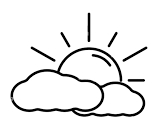
\includegraphics[scale=0.6]{../img/nuvole.png}
\end{center}

Come back to the mountain path.

\begin{itemize}
\tightlist
\item we're walking on the path.
\item the clouds are gathering \(\rightarrow\) signifier.
\item we understand that it's about to rain \(\rightarrow\) signified.
\item we decide to come back to the car \(\rightarrow\) practical effect.
\end{itemize}

Signs often have a practical effect.

Sounds often have a practical effect (hearing thunder is like seeing clouds).

Have music pratical effect?

Signs connect: 
\begin{itemize}
\tightlist
\item something perceptual \(\rightarrow\) the sight of cars or clouds with 
\item something cognitive \(\rightarrow\) the presence of the path or impending rain.
\end{itemize}

Signs are not signifiers \(\rightarrow\) their perception by someone is.

A sign is not something that represents something else.

It represent the relationship someone establishes between two elements:

\begin{itemize}
\tightlist
\item a perceptible dimension (the view of the clouds). 
\item  an intelligible dimension (we connect it to the possibility of rain).
\end{itemize}

This relationship: 

\begin{itemize}
\tightlist
\item occurs \textit{a posteriori}.
\item is not necessarily intentional on the part of the sender (clouds are not harbingers of rain, just as the person who parked on the side of the road didn't mean to tell us the start of the trail).
\end{itemize}
We can connect signifier and signified only through an experiential factor (previously, when we saw those clouds, it rained).

\begin{center}
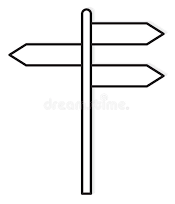
\includegraphics[scale=0.4]{../img/cartello.png}
\end{center}

Signification \(\rightarrow\) as the examples just given, we are constantly surrounded by a multiplicity of unconsciously produced signs.

All these signs have the potential to become signifier expressions if interpreted by a recipient in the general act we can define as signification.

Communication \(\rightarrow\) the sign is voluntarily produced by the emitter to convey a message, such as the signs in the previous image or the same images within this text.

Listen (\href{http://www.musicaecodice.it/gitmedia/emc/1_media/annuncio.mp3}{exemple 1}, \href{http://www.musicaecodice.it/gitmedia/emc/1_media/pubbli.mp3}{exemple 2}, \href{http://www.musicaecodice.it/gitmedia/emc/1_media/ligeti.mp3}{exemple 3}) and answer.

\begin{itemize}
\tightlist
\item what is the practical effect of the three sound texts?
\item is sound information contained in the acoustic properties of the sound texts?
\end{itemize}

Sounds can be both signification and communication.

Music can be only comunication.

In the performing arts of non-oral traditions (such as the western musical tradition), things get even more complicated because several actors play in the communication process:

\begin{itemize}
\tightlist
\item composer \(\rightarrow\) usually thinks of a composition in his mind (symbolic musical language) and then represent it through some kind of notational code on a score.
\item score \(\rightarrow\) the coded instructions needed by an interpreter to reproduce the composer's ideas in the physical world in the form of sound waves.
\item interpreter \(\rightarrow\) must know both the musical language used by the composer and the symbolic language through which it was codified (semiography).
\item listener \(\rightarrow\) receiver that interprets an interpretation.
\end{itemize}

In acoustic music it is always like this, while in electroacoustic music things can change.

\subsection{Do you know this music? }\label{do-you-know-this-music}

\begin{center}
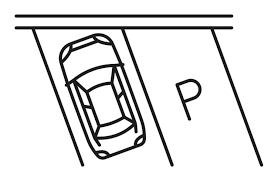
\includegraphics[scale=0.4]{../img/parcheggio.png}
\end{center}

What is the relationship between signifiers and signifieds activated bythe receiver based  on?

Is this relationship always valid and somehow implicit in the signifier, or does it depend on context and conditions?

Let's consider the example of clouds and rain.

There is no an universal law that says that every time there are clouds in the sky, it will rain.

The relationship is established through `a posteriori' inductive generalization codified in an interpretative rule \(\rightarrow\) it often rained after observing clouds in the sky, and therefore, whenever we encounter clouds, we associate them with the phenomenon.

Does this also apply to the example of cars parked on the side of the road?

In this case:

\begin{itemize}
\tightlist
\item there isn't an universal law according to which every time we observe parked cars, a mountain path is nearby.
\item there isn't an interpretative rule established by inductive generalization, since parked cars rarely indicate the start of a trail.
\end{itemize}

The way of reasoning that led to the signification (inference) was induced:

\begin{itemize}
\tightlist
\item by the contingent dimension \(\rightarrow\) place and context.
\item by the affective dimension \(\rightarrow\) enthusiasm for the hike, desire to find the trail to start walking, etc.
\item by the reference culture, or that set of knowledge, value systems, habits, and behaviors within which we live and which have almost naturally led us to that conclusion and not another.
\end{itemize}

The cognitive inferences used daily in our interpretations are not entirely personal or subjective \(\rightarrow\) are based on precise codes.

These codes:

\begin{itemize}
\tightlist
\item are formal systems that transcend individual choices, often imposing the use of certain mental categories.
\item are not universal.
\item are more or less lasting stabilizations of collective ways of thinking, acting, desiring, and preferring.
\item are dictated, maintained, and modified by social pressure.
\item are social and cultural customs, interpretative habits that take on the appearance of a law (without actually being one).
\end{itemize}

If we hadn't shared the same culture and been part of the same society with the many people who parked their cars on the day of the excursion, that sign simply wouldn't exist.

The sign isn't in things or ideas, but in the forms of their relationship.

Listen (\href{http://www.musicaecodice.it/gitmedia/emc/1_media/miles.mp3}{exemple 1}, \href{http://www.musicaecodice.it/gitmedia/emc/1_media/rameau.mp3}{exemple 2}, \href{http://www.musicaecodice.it/gitmedia/emc/1_media/gamelan.mp3}{exemple 3}) and answer.

Describe the differences between the three sound texts: 

\begin{itemize}
\tightlist
\item what is the first information that comes to mind when you listen? 
\item what kind of information is? 
\item are there differences between the linguistic systems used in the three sound texts? \item if there are any, what information do they influence?
\end{itemize}

Some of these arguments lead us to understand sound signs as a cultural phenomenon and not merely acoustic since from this point of view the signifier coincides with the signified.

\subsection{Do you like this music?}\label{do-you-like-this-music}

\begin{center}
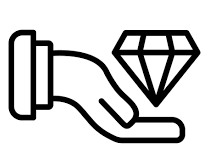
\includegraphics[scale=0.4]{../img/valore.png}
\end{center}

The above codes are anthropological conventions.

The relationships between expressions and content are connected to values, preferences, and tastes, all of which are extremely complex and are:

\begin{itemize}
\tightlist
\item arbitrary \(\rightarrow\) when viewed from the outside.
\item undisputed \(\rightarrow\) when viewed from the inside.
\end{itemize}

A sign arises through difference when a sensorial discontinuity materializes, such as when, while driving along a mountain road, we encounter parked cars.

The perceptual gap brings to the surface something significant, important, which we value by distinguishing it from other signs encountered along the way.

We value it in two ways:

\begin{itemize}
\tightlist
\item we are happy because we have found what we were looking for, namely, the opportunity to embark on a beautiful hike in the mountains.
\item we have achieved what we were seeking through a journey of knowledge that has kept our attention high (observing signs, the environment, other signs, etc.) and evaluating by comparing things (would it be better to stop at a restaurant or go for an hike?).
\end{itemize}

Social codes do not completely transcend individual choices but are linked to the ways in which the individual assumes them by mediating between collective and individual values.

In summary:

\begin{itemize}
\tightlist
\item value is what we aim for and what directs our series of actions and passions, giving precise meaning to each of them according to an implicit path.
\item value arises from the evaluative comparison of things, objects, and from the recognition of differences; the greater the evaluative comparisons along the path, the greater the value.
\item the continuous mediation between collective and individual values \hspace{0pt}\hspace{0pt}generates changes in anthropological codes.
\end{itemize}

Let's see a \href{http://www.musicaecodice.it/gitmedia/emc/1_media/sordi1.mp4}{video}.

\subsection{Texts and narratives}\label{texts-and-narratives}

\begin{center}
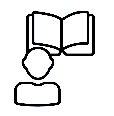
\includegraphics[scale=0.75]{../img/neuro.png}
\end{center}

The sign is just an iceberg tip.

It works because:

\begin{itemize}
\tightlist
\item it breaks down into many small, interrelated elements.
\item it composes larger entities by relating to other similar signs.
\end{itemize}

The parked cars signify the discovery of the path because:

\begin{itemize}
\tightlist
\item their unusual number in that place.
\item the way they are parked on the edge.
\item they thicken as they approach the path and then thin out.
\item they are in that place and not somewhere else.
\item they take on value thanks to differential relationships with other signs.
\item we are looking for the beginning of the path and not something else.
\item all these and other elements are part of a story that unfolds in a precise period of time.
\item this narrative is seen through a specific value-based, cultural, and anthropological perspective (a mountain hike).
\item we are in a specific emotional state (positive tension generated by the anticipation of being able to begin something we enjoy).
\item
  \ldots{}
\end{itemize}

The relationships established between these elements in a narrative generate the code through which that signifier refers to that probable meaning and not to another, forming what we might call a dynamic text.

Signs function because they are intertwined in texts.

The words of a language are like signs:

\begin{itemize}
\tightlist
\item the variable result of constant relationships between smaller elements (morphemes, phonemes, sound features),
\item themselves entities that compose larger structures (sentences, texts, speeches).
\end{itemize}

Every larger element capable of meaning transcends the smaller elements.

The meaning of a sentence transcends the meaning of the individual words that compose it, as well as the individual phonemes.

Texts are not just books, documents, etc., but any portion of the world with:

\begin{itemize}
\tightlist
\item determined limits (context).
\item precise internal articulation (code).
\end{itemize}

that carries some configuration of meaning, or better yet, a signification.

Do you remember the puzzle?

In order for meaning to:

\begin{itemize}
\tightlist
\item be produced.
\item be circulated.
\item be received.
\item be transformed.
\end{itemize}

it must refer to texts or units of meaning that various societies, historical periods, and cultures use to define their core values.

Let's see a \href{http://www.musicaecodice.it/gitmedia/emc/1_media/storia1.mp4}{video}.

\section{Forms of human expression}\label{forms-of-human-expression}

We can summarize the concepts just presented by following the thoughts of the musicologist J.J.Nattiez set out in his text `Music and discourse'.

Forms of human expression (including music) can be defined as symbolic forms only if we recognize three levels:

\begin{itemize}
\tightlist
\item poietic dimension (emitter) \(\rightarrow\) the set of strategies activated by the author that lead to the creation of the work (something that did not exist before).
\item aesthesic dimension (receiver) \(\rightarrow\) the set of strategies activated by the listener during the perception of the work.
\item the work itself (neutral) \(\rightarrow\) the text with its own internal organization that can be analyzed independently from the poietic and aesthesic dimensions.
\end{itemize}

\begin{center}
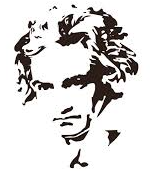
\includegraphics[scale=0.45]{../img/beethoven.png}
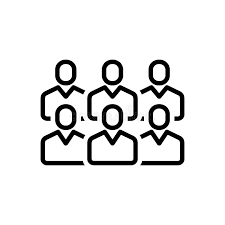
\includegraphics[scale=0.4]{../img/pubblico.png}
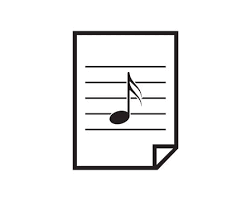
\includegraphics[scale=0.4]{../img/score.png}
\end{center}

\subsection{Poietic dimension}\label{poietic-dimension}

Active process of construction by the emitter (composer) of interpretant signs.

Each sign does not refer directly to an object but makes use of the intermediary action of a second sign which is its interpretant in a process of multiple references.

\begin{center}
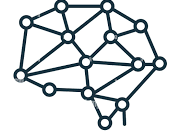
\includegraphics[scale=0.45]{../img/rimandi.png}
\end{center}

For example, in verbal language, if we write a word like table, we have:

\begin{itemize}
\tightlist
\item created a graphic sign (grapheme - formed by a sequence of letters and defined by its own rules) that, if
\item correctly interpreted by the reader, will cause him or her to pronounce the corresponding word (morpheme - sequence of phonemes defined by its own rules). If
\item correctly interpreted by the hearer, it will refer to a general idea of a table (an abstract concept defined by conventions derived from collective experience). If
\item correctly interpreted by someone, it will connect it to a real, meaningful table (object - defined by subjective experience).
\end{itemize}

This is true for a single word.

The interpretative signs become infinite when individual words are organized into a language.

Ognuno sta solo sul cuor della terra trafitto da un raggio di sole: ed è subito sera

Let's try to imagine the same process in music and the amount of control the composer can have over the \href{http://www.musicaecodice.it/gitmedia/emc/1_media/goldberg.mp3}{sound information} he wants to transmit.

\subsection{Aesthesic dimension}\label{aesthesic-dimension}

Active process of construction by the interpretant.

Process of understanding that can be defined as sharing information on cultural operations typical of a human social group.

In the case of artistic languages, the interpretative signs attributed to the work by the emitter are not necessarily the same as those projected by the receiver because:

\begin{itemize}
\tightlist
\item they are modulated by the context in which the interprete perceives the work.
\item they are modulated by any discrepancy in period or cultural context between the emitter and the receiver.
\item the perception of a sonata in the Baroque era is presumed to be totally different from the perception of the same work today, as the historical, social, technological, and cultural contexts are significantly different.
\end{itemize}

\begin{center}
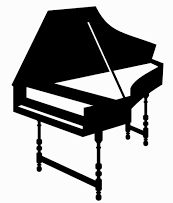
\includegraphics[scale=0.45]{../img/barocca.png}
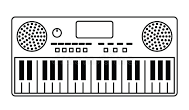
\includegraphics[scale=0.65]{../img/moderna.png}
\end{center}

The perception of a Beethoven symphony by an Amazonian native is totally different from ours, as is our perception of the microtones present in the \href{http://www.musicaecodice.it/gitmedia/emc/1_media/muezzin.mp3}{muezzin chants}.

\begin{center}

\includegraphics[scale=0.6]{../img/indigeni.png}
\end{center}

Let's also think about the technological dimension: the perception of the same sound text in a live concert is different from the perception of its reproduction recorded by an electroacoustic system perhaps while we wait for the subway.

\begin{center}
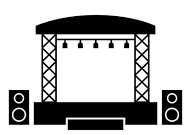
\includegraphics[scale=0.5]{../img/acousma.png}

\includegraphics[scale=0.5]{../img/sony.png}
\end{center}

\subsection{The work itself}\label{the-work-itself}

Regarding the understanding of the sound text itself Nattiez advocates the need to analyze: 

\begin{itemize}
\tightlist
\item works and styles as cultural and anthropological objects. 
\item harmony, rhythm, meter and all aspects that have a similar function in the grammar of natural language (comparison).
\end{itemize}

When we speak of grammars of musical parameters we are not referring exclusively to the analysis of the formal and structural characteristics of a specific musical text. We must also take into consideration the grammars of musical parameters generalized and historicized in styles and forms.

\begin{center}

\includegraphics[scale=0.45]{../img/trattato.png}
\end{center}

Nattiez borrows from the study of verbal language the semantic exercise of breaking down meaning according to the use of words, which in music corresponds to the analysis of a melodic profile or a rhythmic system, or the distribution of harmonic fields in a tonal system or twelve-tone series, etc.

\begin{center}
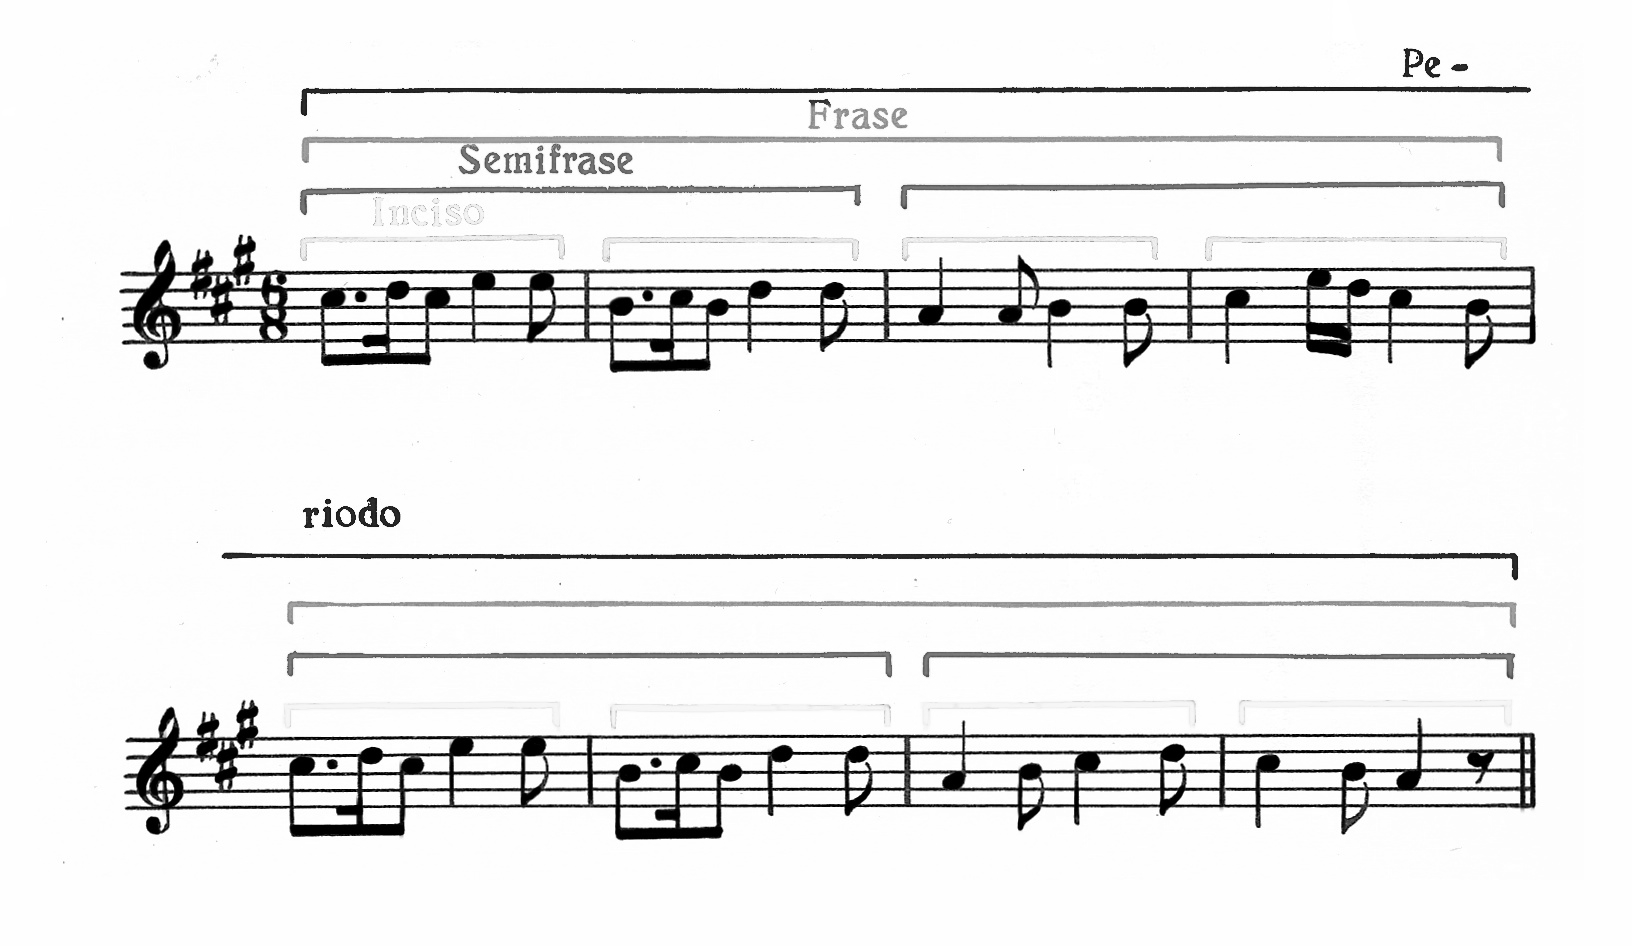
\includegraphics[scale=0.85]{../img/frasemus.png}
\end{center}

Each musical element (pitch, intensity, duration, timbre) can be separated and taken as a strategic variable in the production of a \href{http://www.musicaecodice.it/gitmedia/emc/1_media/quinta.mp4}{musical work}.

Ending, for Nattiez constructing a musical theory is the organization of a selection of interpretants adopted within an anthropological context.

Anyone who wants to invent a new musical grammar (a practice that has been widespread among art music composers since the 1950s) must take this into account and not just the definition of rules internal to the text.

Works do not exist in isolation since it is their place in history that provides their meaning and possible interpretations over time.

\begin{center}
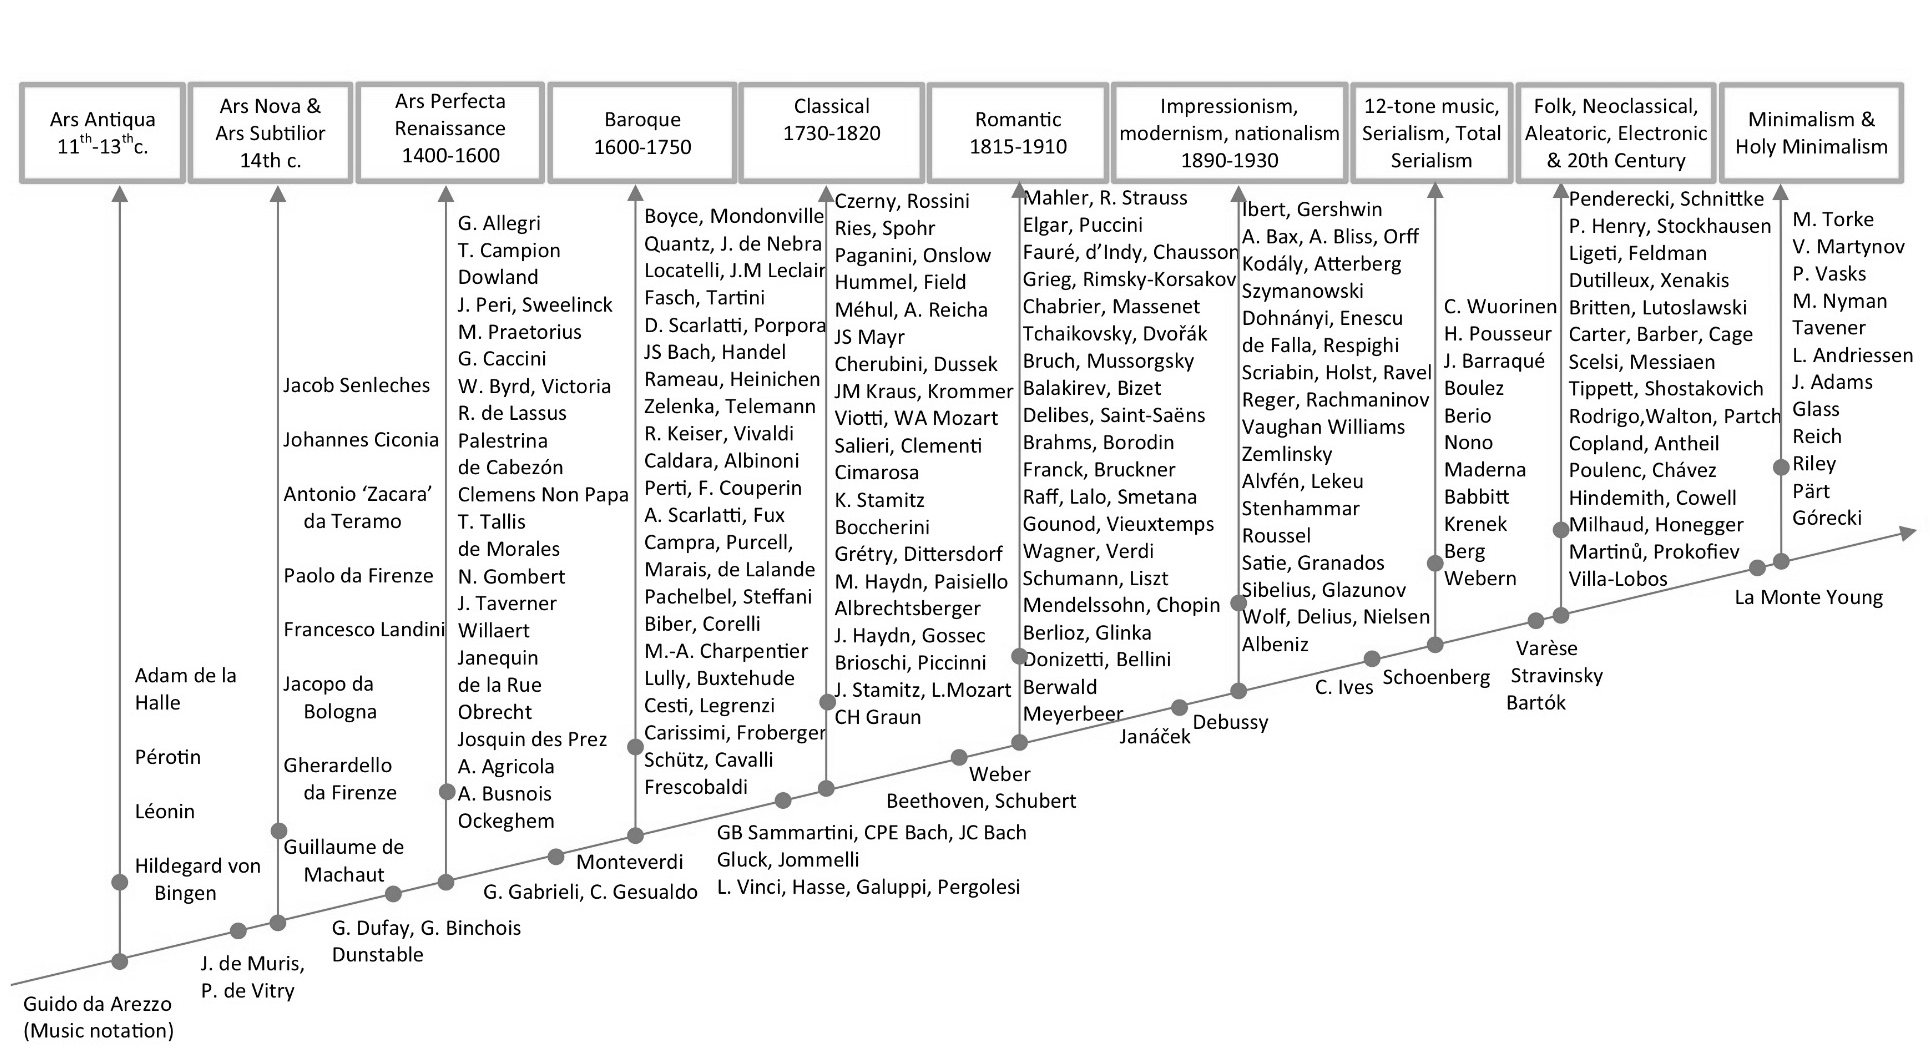
\includegraphics[scale=1]{../img/lineatempo.png}
\end{center}

The sound text can live a life of its own and be isolated from the the emitter but not from the anthropological context in which it was created and/or reproduced.

\subsection{Final reflections}\label{final-reflections}

Everyday life is filled with more or less voluntary signification.

Signification is the amniotic fluid within which human beings live.

We can highlight it and clarify its mechanisms.

This task is often hidden in everyday life.

For example, if we ask someone why they like a piece of music or a dress they will probably answer:

\begin{itemize}
\tightlist
\item because it's beautiful.
\item because it excites me.
\item because it's right.
\item because\ldots{}
\end{itemize}

Meaning often hides behind other motivations that tend to suppress it.

Let's think about written and spoken language.

In using it, we put into practice extremely complex knowledge that we tend to be unable to explain.

We would hardly be able to fully explain all the grammatical, phonetic, morphological, and syntactic rules we apply daily.

Language is practical knowledge that we almost never reason about (unless we are professional linguists).

Our daily experience works the same way: it appears random, spontaneous, and immediate.

In reality it is based on a dense and constantly changing network of relationships between things, people, places, etc.

Also the act of composing a piece of music should develops in the continuous passage from awareness of linguistic mechanisms (intelligence) to creativity.

Let'see a \href{http://www.musicaecodice.it/gitmedia/emc/1_media/senso1.mp4}{video}.